\chapter{Background}
\label{chap:bg}
This chapter is divided into two sections. The first one, 2.1 \fixme Theoretical Background,
will provide a description of a simple CPU architecture which focus on the parts used
for executing memory instruction stores. This will be followed by a introduction of
the four already implemented prefetching strategies. Section 2.2 \fixme will go thought the
work flow of this thesis and introduce the tools that are used, modified or created, as
well as how they are combined.
\THsec{Theoretical Background}{ThB}

\THsub{A theoretical Architecture}{TA}
\fixme
\begin{figure}[h]
\centering
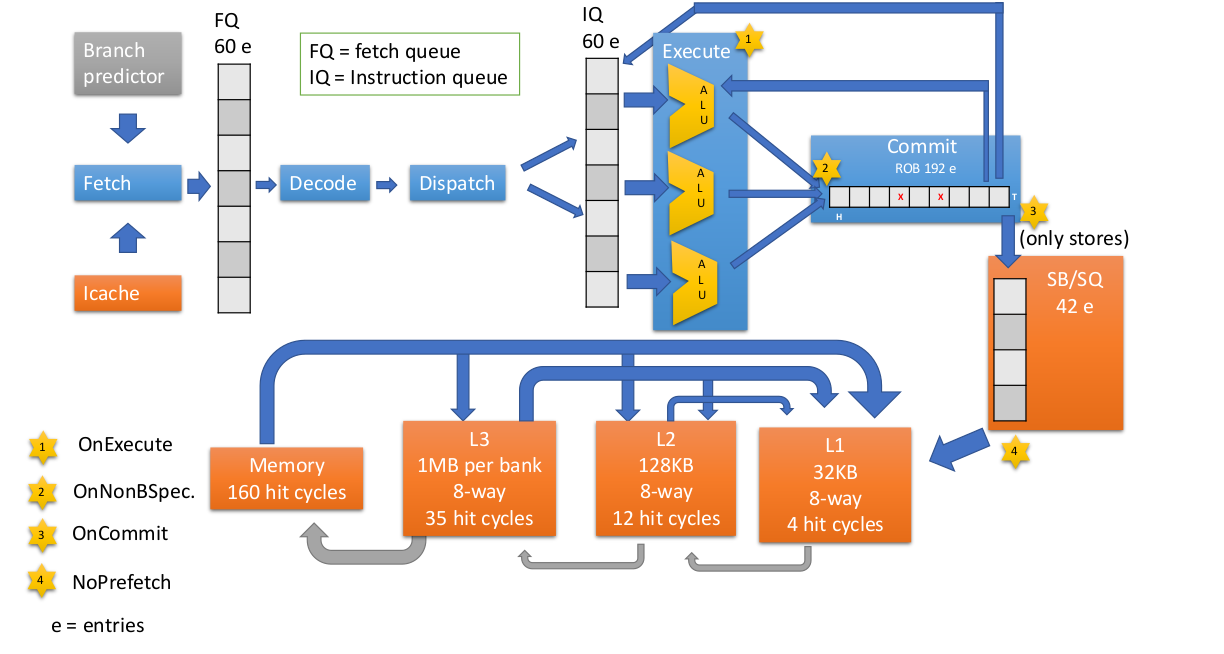
\includegraphics[width=8cm]{figure/thoeratical-arc.PNG}
\caption{Our architecture}
\label{img:arc}
\end{figure}
\\ \\
In the image 2.1 \fixme you see the architecture in use. This images symbolizes almost all
the features and parts of the CPU that will be discussed and analyzed from different
perspectives. If there is a picture that you should keep in mind when reading this
report then this would be it. The stars symbolizes where a prefetch is issued for the
three simplest and already implemented store prefetch policies in 2.1.2 \fixme as well as one
of the proposed once namely NonBSpeculative. The numbers is the one used for the
simulated CPU (see section 3.3 \fixme). In modern CPU’s there are often more then one
core which all have a process pipeline with several stages. The pipeline is split in
stages to increase the throughput of executed instructions. One can compare it with
a car factory where the car travels on a conveyor belt through different stations and
on each station something is done with the car, i.e. seats, wheels or the engine can
be installed.
\\ \\
The CPU to be simulated have a five stage pipeline. As going through the stages,
some key parts of the CPU will be introduced. One thing to mention before moving
on is that the CPU will execute instructions out of order but it promise that the effect
will always be like if the instruction where executed in order.
 \\ \\

\THstage{Fetch}
A new instruction (see 3.4 \fixme) will be added to the processor. In the basic case the
next instruction will be brought in from the \THnewWord{Icache} (Instruction cache). Icache is
a L1 \THnewWord{cache} the holds the instructions to be executed in the near feature trace ref.
The CPU has a \THnewWord{PC} (program counter) which keeps track of the address of the current
instruction that is fetched, when fetching the next instruction the PC will be
incremented by the length of the current instruction. Caches will covered in 2.1.1. \fixme
Different loops are widely used in programming and a loop tells us if we should go
back to the beginning of the body of the loop or if the loop should be terminated
and the lines below should be executed. A CPU cannot for example execute C code,
it needs to be compiled first. Compilation is a translation from code to instructions
within the instructions set that are supported by the CPU in question. A loop will
be compiled to a branch instruction which will have the target instruction address
and the condition to be satisfied if the branch is taking (take one more lap in the
loop). The problem is that we want to continue to bring in new instructions before
the condition have been computed, but which instructions will be next. Here comes
the \THnewWord{Branch predictor} to use, it predicts the outcome of a branch and make the CPU
able to load instructions based on that prediction. If a branch is taken the PC is set
to the branch target address. If a prediction turn out to be wrong the CPU will remove
the work and all the side effects produced by the wrongly executed instructions.
Fetched instructions will be placed in the fetch queue (our has 60 entries).

\THstage{Decode}
The instruction (from the instruction queue) will here be interpreted.
\THstage{Dispatch}
In this stage we take care of dependencies. If we want to add two numbers and
then multiply the result with a third number, then the addition has to be finished
before the multiplication can be executed, thus the multiplication has a dependency
to the addition. If we also have to store the result of the multiplication then the
multiplication needs to be computed before we can store the result of it. This gives a
dependency between the store and the multiplication. When the dependencies have
been worked out, the instructions will be put in the \THnewWord{Instruction queue} (IQ) (who
has 60 entries as well).

\THstage{Commit}
Commit is the last step of the pipeline and it contains a ROB (ReOrdering Buffer)
with 192 entries. This buffer puts the out of order executed instructions back into
order. This means it is possible, given just the ROB, to execute 191 instructions ahead
while waiting on an instruction to be finish. When all instructions in a sequence are
done they can leave the pipeline. The {\color{red}x} in figure 2.1 \fixme illustrates a squashed instruction,
if a branch prediction turns out to be wrong then we need to squash all the instruction
that should never have been executed but have been based on that faulty prediction.
Going back to the example with the sum of two number multiplied by a third number.
When the addition is done and the result is added to the ROB, the multiplication
instruction in the \THnewWord{IQ} (Instruction Queue) is informed that its dependent instruction
is done (the arrow from ROB to IQ in figure 2.1\fixme). Finally the arrow from ROB to
ALU will provide the result from the addition to the multiplication.
\THstage{SB}
The path that have been described until now is taken by every instruction but now
we will continue the way that store instructions are taken. When a store instruction
leaves the ROB it comes to the \THnewWord{store buffer} (which can also be called store queue):
The store instruction is here represented in terms of the memory address to be fetched
and the data to be stored. The buffer is FIFO-ordered (first in first out), the first
store in the buffer sits and waits for its data to be ready in the L1 cache (see 2.1.1)
and blocks all operations behind in the buffer. This is the means that the buffer only
interact with the L1 cache.
\THsubsub{Memory and caches}
The memory structure (in the center of figure \ref{img:arc}) is of course a key part when talking
about store instructions. We begin with the main memory that have a storage capacity
of some gigabytes, a latency of 160 cycles if a hit, and sits on the mother board. Then
we have the cachees, which are placed on the CPU chip. A cache is a quick and small
memory unit in which the data that are likely to be used in the near feature is placed.
In this case we have three which are named L1 (32kiB 8-way 4 hit cycles), L2 (128kiB
8-way 12 hit cycles) and L3 (1MB per bank 8-way 35 hit cycles). Where L stands for
level and the greater the digit, the bigger the cache is and the further away from the
core it is placed. A bigger cache means that it takes longer time to find certain data
in it. The time is measured in \THnewWord{cycles}, in every cycle something can occur in the CPU
i.e. a instruction can be placed in FQ and/or another one can be placed in the ROB.
If our CPU runs in a frequency of 2.2 GHz, there are:

$$ 2.2 \times 1000^3 = 2.2 \times 10^9 cycle / secound$$

Given that one cycles takes:

$$ \frac{1}{2.2 \times 10^9 } = 2.2 \times 10^{-9}s = 2.2ns$$

This give us that it takes: $4 \times 2.2 = 8.8ns$ to retrieve data from the L1 cache. A
cache keeps copies of needed data and the data will be saved in different regions in
the cache depending on the address of the data. The number of ways a cache have
is the number of data shanks in every address range that can be kept simultaneously
in the cache. A larger number of ways means that it takes longer time to determent
if a certain data is present in the case. A smaller number of ways increases the risk
of conflict misses, that is when the cache runs out of places for data from a specific
address range. Our caches are all 8-ways which means that a piece of data can be find
in one of eight places (if it is in the cache) and that a cache can hold no more then
eight data chunks from a given address range. The Icache is like another L1 cache
that only holds instructions, the L2 and L3 cache holds both data and instructions.
When data is loaded into the L1 cache from the main memory it will often be loaded
to all the other cachees at the same time.

\THsub{State-of-the-art of prefetch policies}{GPP}
The question for this master thesis is when to prefetch data into the L1 cache to
minimize the time a store instruction has to wait in the first place of the store buffer.
Three approaches are already implement in the Gems simulator 2.2.3 \fixme and are covered in the literature,  these will
be described and their pros and cons while be mentioned below, based on the architecture
introduced in section 2.1.1. \fixme. These three polices will also be referenced to as "the basic three policies". The starts mentioned in the paragraph headings
are the once in figure \ref{img:src}
\THpar{OnExecute (star 1)}{ONEX} This is the earliest and most speculative one, where the
operation to brought memory into the L1 cache is issued in the execute stage. This
ensure that the data arrives in L1 before it is needed, i.e. its instruction is first in the
buffer. The downside is that several things with impact on the data to be prefetch can
occur. First, if the store instruction is affected by a branch, that branch can turn to
be misspredicted which means that we waste energy and space in the small L1 cache
by bringing in unneeded data. Bringing in data to a cache can cause an eviction of
other data. If a store instruction arrives to the first place in the buffer and found that
its data have been evicted from the L1 cache it have to wait for the data to be brought
to the L1 again. This will hopefully take less time since the data can be left in the L2
cache and be brought from it instead of the main memory. Given that the prediction
is right we might still be in trouble, since when we issue the prefetch, the instruction
have to finish the pipeline and passes through the queue in the buffer. This might
take a long time. During the time the data can have arrived to the L1 buffer and been
evicted due to lack of space since more data have been prefetched from the point in
time it arrives in L1 until the instruction is first in the buffer. A too early prefetch
can also be a vulnerability since malicious software can cause a prefetch of illegal data
before the core figures out that it is illegal, and when it does the data have already
been exposed. To conclude: one can say that this alternative is the best if nothing
goes wrong but it is a lot of things that can go wrong. OnExecute has proposed in a
paper by Kourosh Gharachorloo and Anoop Gupta and John Hennessy. [8]\fixme
\THpar{OnCommit (star 3)}{ONCO} Here the prefetch is issued in the commit stage (when passing
the instruction to the store buffer). This means that unneeded data will not be
prefetched. There is still a possibility that the data while be brought in and evicted
due to lack of space, while waiting, as describe in the previous paragraph. Prefetching
data on commit might still mean that the instruction may be waiting in the first line
of the buffer. This can, in the worst case, fill up the entire buffer which can stall the
processor i.e. block it from executing any other instruction. OnCommit is used by
Intel 64 and IA-32 Architecture [10]\fixme. (They do not use the name OnCommit but they
quickly describe a load prefetch with the following sentence: ”Reading for ownership
and storing the data happens after instruction retirement and follows the order of
store instruction retirement.” ”Reading for ownership” is the same as prefetch with
write permissions and ”instruction retirement” is another name for ”instruction commit”.)
To conclude, OnCommit is the man in the middle between the two extremes,
OnExecute \ref{par:ONEX} and NoPrefetch \ref{par:NOPF}.

\THpar{NoPrefetch (star 4)}{NOPF} Here we have no prefetch, the data will be brought into the
L1 cache then the instruction is first in the buffer. The data we brought will be
needed and not evicted before use, this waste no energy. The downside is that every
instruction will be blocking the buffer for a long time waiting on its data to become
available in the L1 cache. The risk for filling up the buffer and stall the processor
(see 2.1.2 \fixme) is high. To conclude: this is the most energy efficient but the most time
consuming trade off. Upon analyzing the source code of Gem5 [6] \fixme it was discovered
that NoPreftch was the default implemented policy (during the work of this thesis all
other prefetch policies was implemented as well).


\THsec{Simulation infrastructure}{siminf}
Below the used tools which are provided by the supervisor, Albert Ros Bardisa, are
covered. The one that are modified or created within the work of this master thesis
are to be found in chapter 3.\fixme
\THsub{Benchmarks}{benchmarks}
To examine how a CPU behaves and how a memory prefetching approach will work
one have to run, or in this case simulate the run of a program. This is often called
benchmark. For this work the SPEC CPU \textcopyright 2016 industry-standardized benchmark
suite [3] \fixme was used. It is designed to stress both the CPU and the memory subsystem
and consists of 55 different benchmark programs that have been used to evaluate the
different prefetch policies.
\THsub{Sniper}{sniper}
Sniper is a parallel, high-speed and accurate x86 simulator with support for multicore
according their web page [2] \fixme. Sniper takes two things as input, a bunch of configurations
that describes the architecture to simulate, and a command line with the call to
the application which we want to simulate, for example one of the programs in 2.2.1.
Sniper can then produce graphs and other document that describes and measures the
simulation of the chosen program on the chose CPU configuration. Two examples of
plots that can be generated is CPI stacks [1] and energy stack which are bar diagrams,
with one bar per thread in the program. The bars are divided in different regions
based on the percentages of time or energy spent in that region. The region can be:
Ifetch, mem-l1, mem-l2 or branch.
\THsub{GEMS}{GEMs}
The Wisconsin Multifacet Project at the university of Wisconsin have released a General
Execution-driven Multiprocessor Simulator (GEMS). The simulator is written in
C/C++ and is an open-source software. The version used in this work was provided
by my supervisor (Albert Ros Bardisa) who had implemented the three basic prefetch
policies (NoPrefetch, OnCommit and OnExecute) along with one that he have come
up with but not publicized (OnNonBSpeculative) as well as support for the changes
to the traces in Sniper that was done during this thesis (see 2.2.2)\fixme. Support for the
policies to be proposed in this work was implemented based on the received source
code.
GEMS takes a path to a folder containing traces (like in 3.4)\fixme, an array of configuration
settings (see 3.2 and 2.1)\fixme and a path for writing the output stats-file. A
stats-file consist of around 2000 lines and are divided into two part, a configuration
part were you find the information given to GEMS in the configuration array and
a Stats part with a lot of measurements like number of cycles and the number of
accesses to the caches, to just mention tWo of them.
